% ----------------------------------------------------------------------------------------
% CHAPTER TITLE
% ----------------------------------------------------------------------------------------
\chapter{Experimental electronic systems in the musical arts: design concepts and history}\label{background}
\lhead{\chaptertitlename\ \thechapter. \emph{Background}}
% ----------------------------------------------------------------------------------------
\begin{quote}
	
	...not as descriptive of an act to be later judged in terms of success and failure, but simply as of an act the outcome of which is unknown. 
	
	\cite[p.13]{cage1961}
	
	\end{quote}
	
If experimental music is an act of uncertain consequences, transferring the concept over to engineering appears as counterintuitive. Great effort goes into making commercial electronics consistent, predictable and uniform. The same largely holds for electronic instruments - ``one-offs" with unpredictable behaviors or cryptic functions drastically reduce the overall adoption of the device, and therefore, their commercial potential \cite[p.5]{haslett2005}. In this context, the gap between the determinism of product design and the desire for originality of musical performances is bridged by the musician. ``Finding your sound" is about finding an instrument and using it effectively.  

Making, modifying or otherwise altering electronics is one option to better understand the tools at their disposal and make the most of them. Numerous historical precedents for personalized instruments will be presented in the upcoming chapter, while contemporary instances will be developped in the next. All of them were developed out of a concern for originality, costs, or simple curiosity. Throughout those examples, we'll see how electronic instrument design practices have developed from the example set by the electron pioneers, explored the different levels for experimentation within that space, and how those modern practices converge with contemporary digital technologies. By becoming more accessible to the general public, these technologies bring electronic instruments towards an increasingly personalized musical field of expression \citep{hermans2014}.

\section{An organology of electronic instruments?}  

The development of electronics defined what could be done by artistically-inclined tinkerers, while pre-existing instruments and musical traditions shaped what those tinkerers implemented. The influence of acoustic music traditions is still clearly visible on electronic music today. One could consider the electronic instruments to be a continuation of and response to the acoustic music. 

The fabrication of acoustic instruments is a craft. Organology, formalized in 1914 by the Hombostel-Sachs system \citep{von1961}, was an attempt at classifying musical instruments of the time. By considering the mechanical differences between each instruments, the system separated music-making devices into four categories: 

\begin{itemize}
	\item idiophones, or self-supporting vibration systems
	\item membranophones, with a vibrating membrane
	\item chordophones, using vibrating strings
	\item aerophones, relying on vibrating volumes of air
\end{itemize}

The materials and their geometry clearly define a mechanism, and that mechanism defines the instrument. This is a purely physical parameter space, which takes advantage of the complexities of the real world to develop sophisticated systems. Classification helps exploration: organology provides a context within which a luthier could easily understand the boundaries of their craft. 

What separates acoustic and electronic instruments is also what limits organological classification. Indeed, it is difficult to expand to electronic instruments because the physical phenomena behind oscillations (sound) in these instruments is more difficult to categorize. In attempts to modernize organology, electronic instruments are simply designated as electrophones \citep{hugill2012}. As Hugill notes, this system does not give justice to categories such as extended acoustic instruments, gestural interfaces, and infra-instruments \citep{bowers2005}. It appears difficult to design a robust classification system without shifting from a focus on mechanical engineering to an approach referencing electrical and mechanical systems equally \citep{haslett2005}. 

	Although instrument design could still be considered a craft, electronic music drastically redefined the concept of what an instrument could be and how it could be conceptualized \citep{pinch2002}. This discussion focuses on the expanded skillset that comes with the introduction of electro-mechanical hybrids in the matter of creating sound, and exposes some of its consequences for the silicon luthier. 

\section{Circuit design. innovation at multiple levels: component, system, interaction}

The design parameters of electronic instruments is a newer space, defined by the electronic components available. This has two consequences for every electronic instrument maker since the rise of publicly available electronics in the nineteen-twenties:

\begin{itemize}
	\item electronic instrument and their pre-manufactured electronics offer an additional degree of separation from the organic world. 
	\item design plans go from being a representation of the final product to an schematic abstraction. The two offer different liberties in the fabrication process.
\end{itemize}
	
The question of experimentalism in electronic music hardware implies the following: to what extent has the standardization of resistors, capacitors and other basic electric building blocks standardized the space of possibilities for electronic music instruments?

To better discuss the world of audio electronics design, let us introduce some basic concepts involved in those processes. The design of instruments includes elements of electrical engineering and product design, both of which can be informed by some musical tradition or system. A completed schematic gives enough information to reproduce a device, often complimented by a bill of materials, a circuit board etching plan, and a diagram for the physical layout of parts. In case of a digital device, some component will be a microcontroller loaded with executable code. 

\begin{figure}[h!]
  \caption{schematic of tube preamplifier designed by the author}
  \centering
    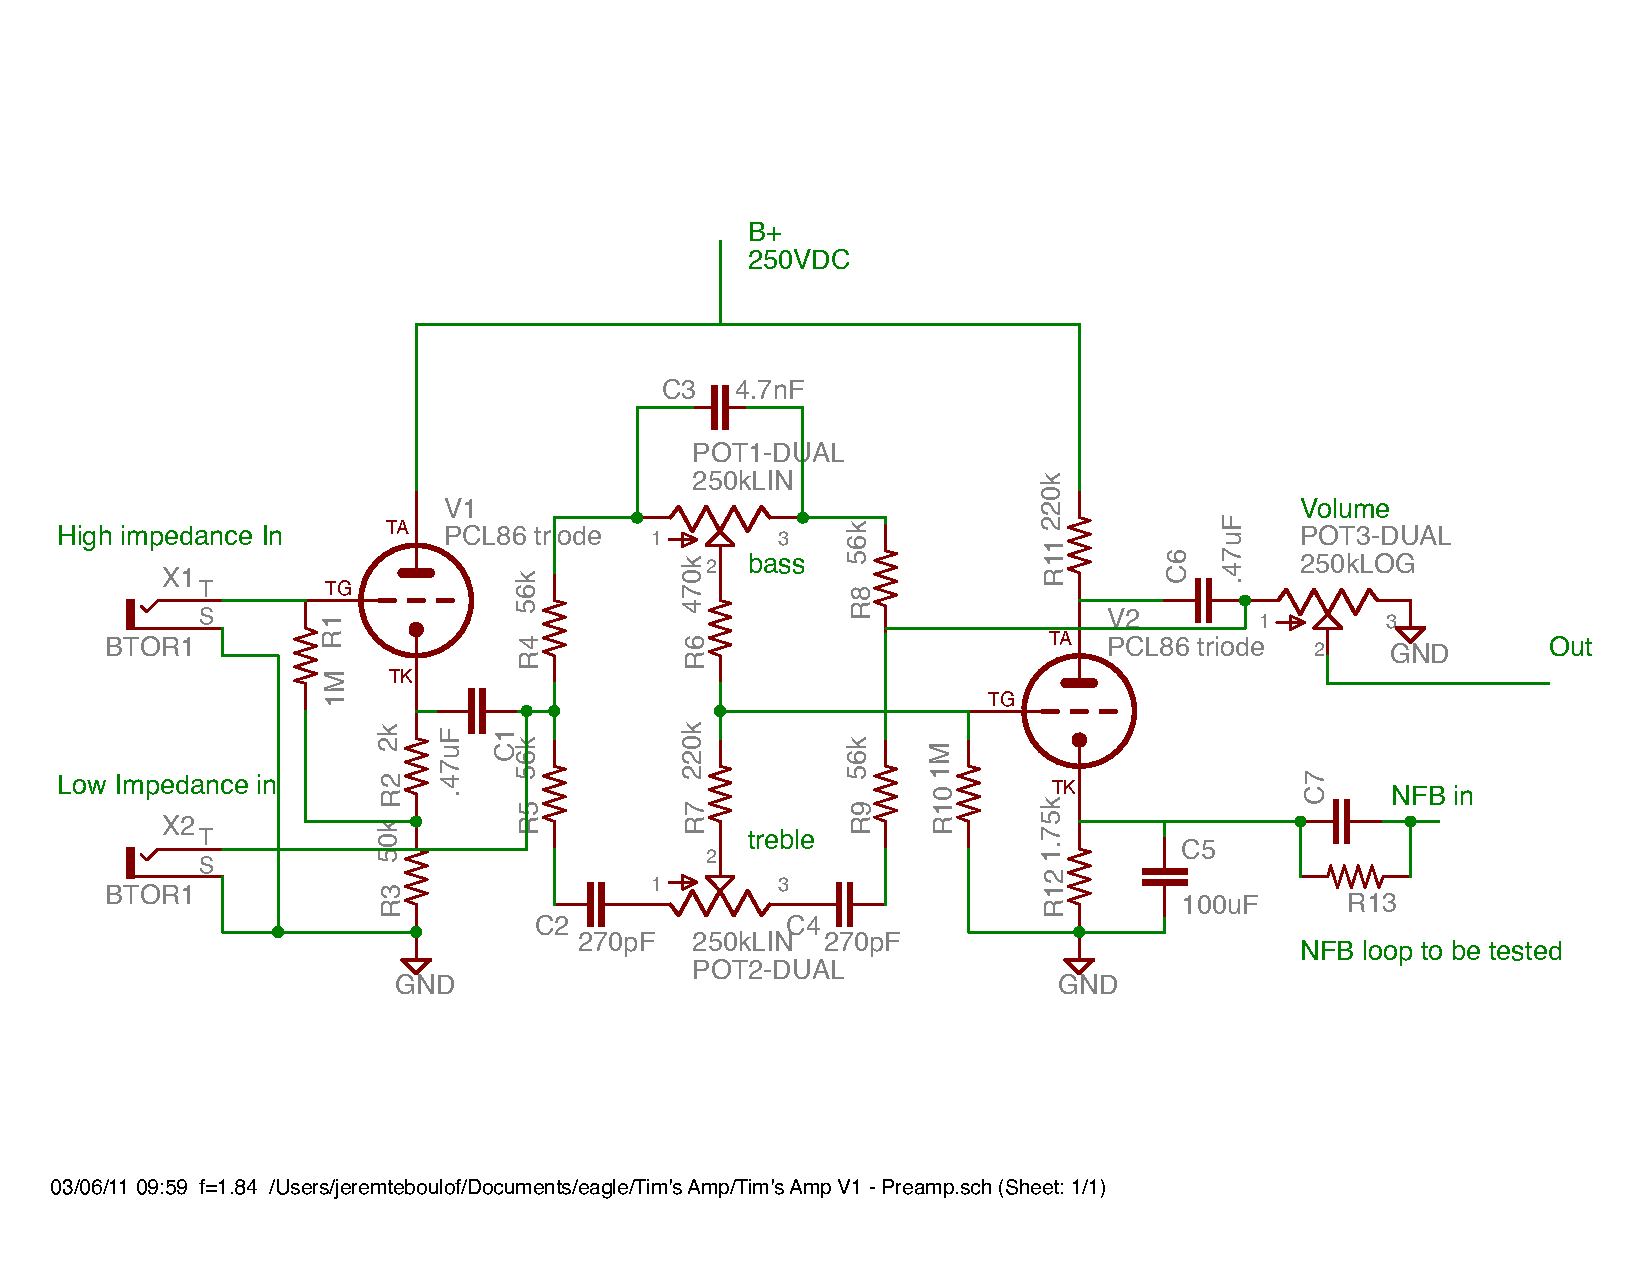
\includegraphics[width=1\textwidth]{timsamp}
\end{figure}

\begin{figure}[h!]
  \caption{bill of materials for that preamplifier}
  \centering
    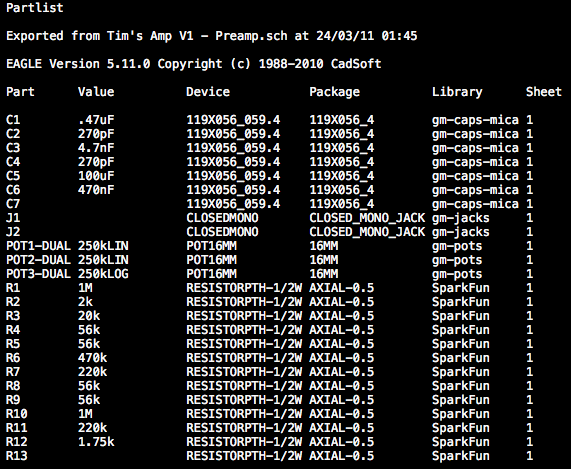
\includegraphics[width=1\textwidth]{bompre}
\end{figure}

The ubiquity of digital devices today cannot be overstated. This is particularly true in musical devices - the versatility of artistic computing is discussed at length by musicians in the upcoming chapters. 

Software design offers a rich tradition of experimentalism for audio. Max Mathews acts as the forefather of a long line of extensively-studied composers who either programmed their own instruments, or worked closely with engineers to do so. Those efforts effectively redefined the world of electronic music, and as we'll see excluding digital from a discussion of contemporary audio hardware in music would be as toxic as it would be difficult. Open source originates in software- this thesis wishes to expose the possibilities of interdisciplinary design approaches. 

	By looking at the role of experimentalism in electronic music hardware, one can get a sense of how hardware can complement the speed of innovation that characterizes software. Improving physical music devices can take three forms:  
	
\begin{itemize}
	
\item component innovation

\item system innovation 

\item interaction innovation  

\end{itemize}

Historically, electrical engineers have been concerned with those first two points, while the latter is more open to interpretations from various sources. The New Interfaces for Musical Expression (NIME) conference has developed out of a desire to unite efforts in that field. Software affects all three levels, blurring the distinction between component and system while re-labeling interaction design as UX/UI design (user experience/user interface). 

Looking at the historical development of those three types of innovation in electronic music and electronics gives us a better sense of where the field is today. 

\section{Electronic music as invention}

	Before 1915 and the beginning of commercially available vacuum tubes, electronic music relied on a spirit of adventure and experimentalism close to the later works of Tudor, Kuivila, Collins and Ghazala. Dunn's pioneers developed system because they invented or developed interesting forms for the basic components of an electronic circuit (the resistor, the capacitor, the inductor). 
	
\paragraph{Thomas Edison}

	\begin{figure}[h!]
	  \caption{one of Edison's ``Tone Tests'', 1918 \cite{thompson1995}}
	  \centering
	    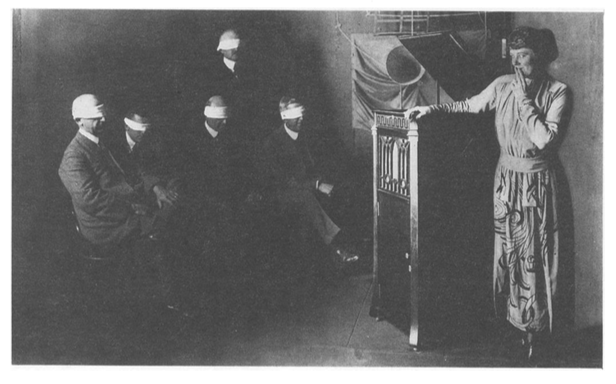
\includegraphics[width=.5\textwidth]{tonetest}
	\end{figure}
	
Edison was, in addition to his involvement in the electrification of western countries in the early 20th century, an accomplished inventor and tinkerer. The phonograph he toured to advertize in the United States through \emph{tone tests} emphasized the intelligibility of the voices it reproduced. Although critics pointed out the impressive but imperfect reproduction from the device, Edison maintained that they couldn't accurately distinguish one from the other \cite{thompson1995}. 

There could not have been a better link between Aristotle's acousmats and Schaeffer's listening techniques - and this context sets the framework within which electricity and music would live up to this day. It is difficult to imagine or think of the synthesized without referring to the ``natural'', almost as it is easy to disregard the point or the honesty of electronic instruments. And yet, purely electrical instruments developed. Whether by accident, rigorous research, or haphazard guesses, the early inventors of electronic music were also trying to convince others that their work was, at the very least, asking interesting questions. 
	
\paragraph{C.G. Page}

	C.G. Page “toyed” with horseshoe magnets, spools of copper wire and batteries - in 1837, he would publish one of the first reports of electronic sound, which he called galvanic music without being able to explain it \citep{page1837}. 
	
\paragraph{Elisha Gray}

	Elisha Gray, in 1874, was the first electronic musician to tour his home country. His invention, the musical telegraph, was invented after he realised he could control the pitch of the hum produced by a vibrating metal strip attached to his bathtub while running experiments with his nephew. After touring once with it, he ignored its musical potential and failed when he attempted to use a modified version of the device as an early iteration of what would then become the multiplexer \citep{holmes2002}. 
	
	\begin{figure}[h!]
	  \caption{Gray's Electro Harmonic Telegraph patent}
	  \centering
	    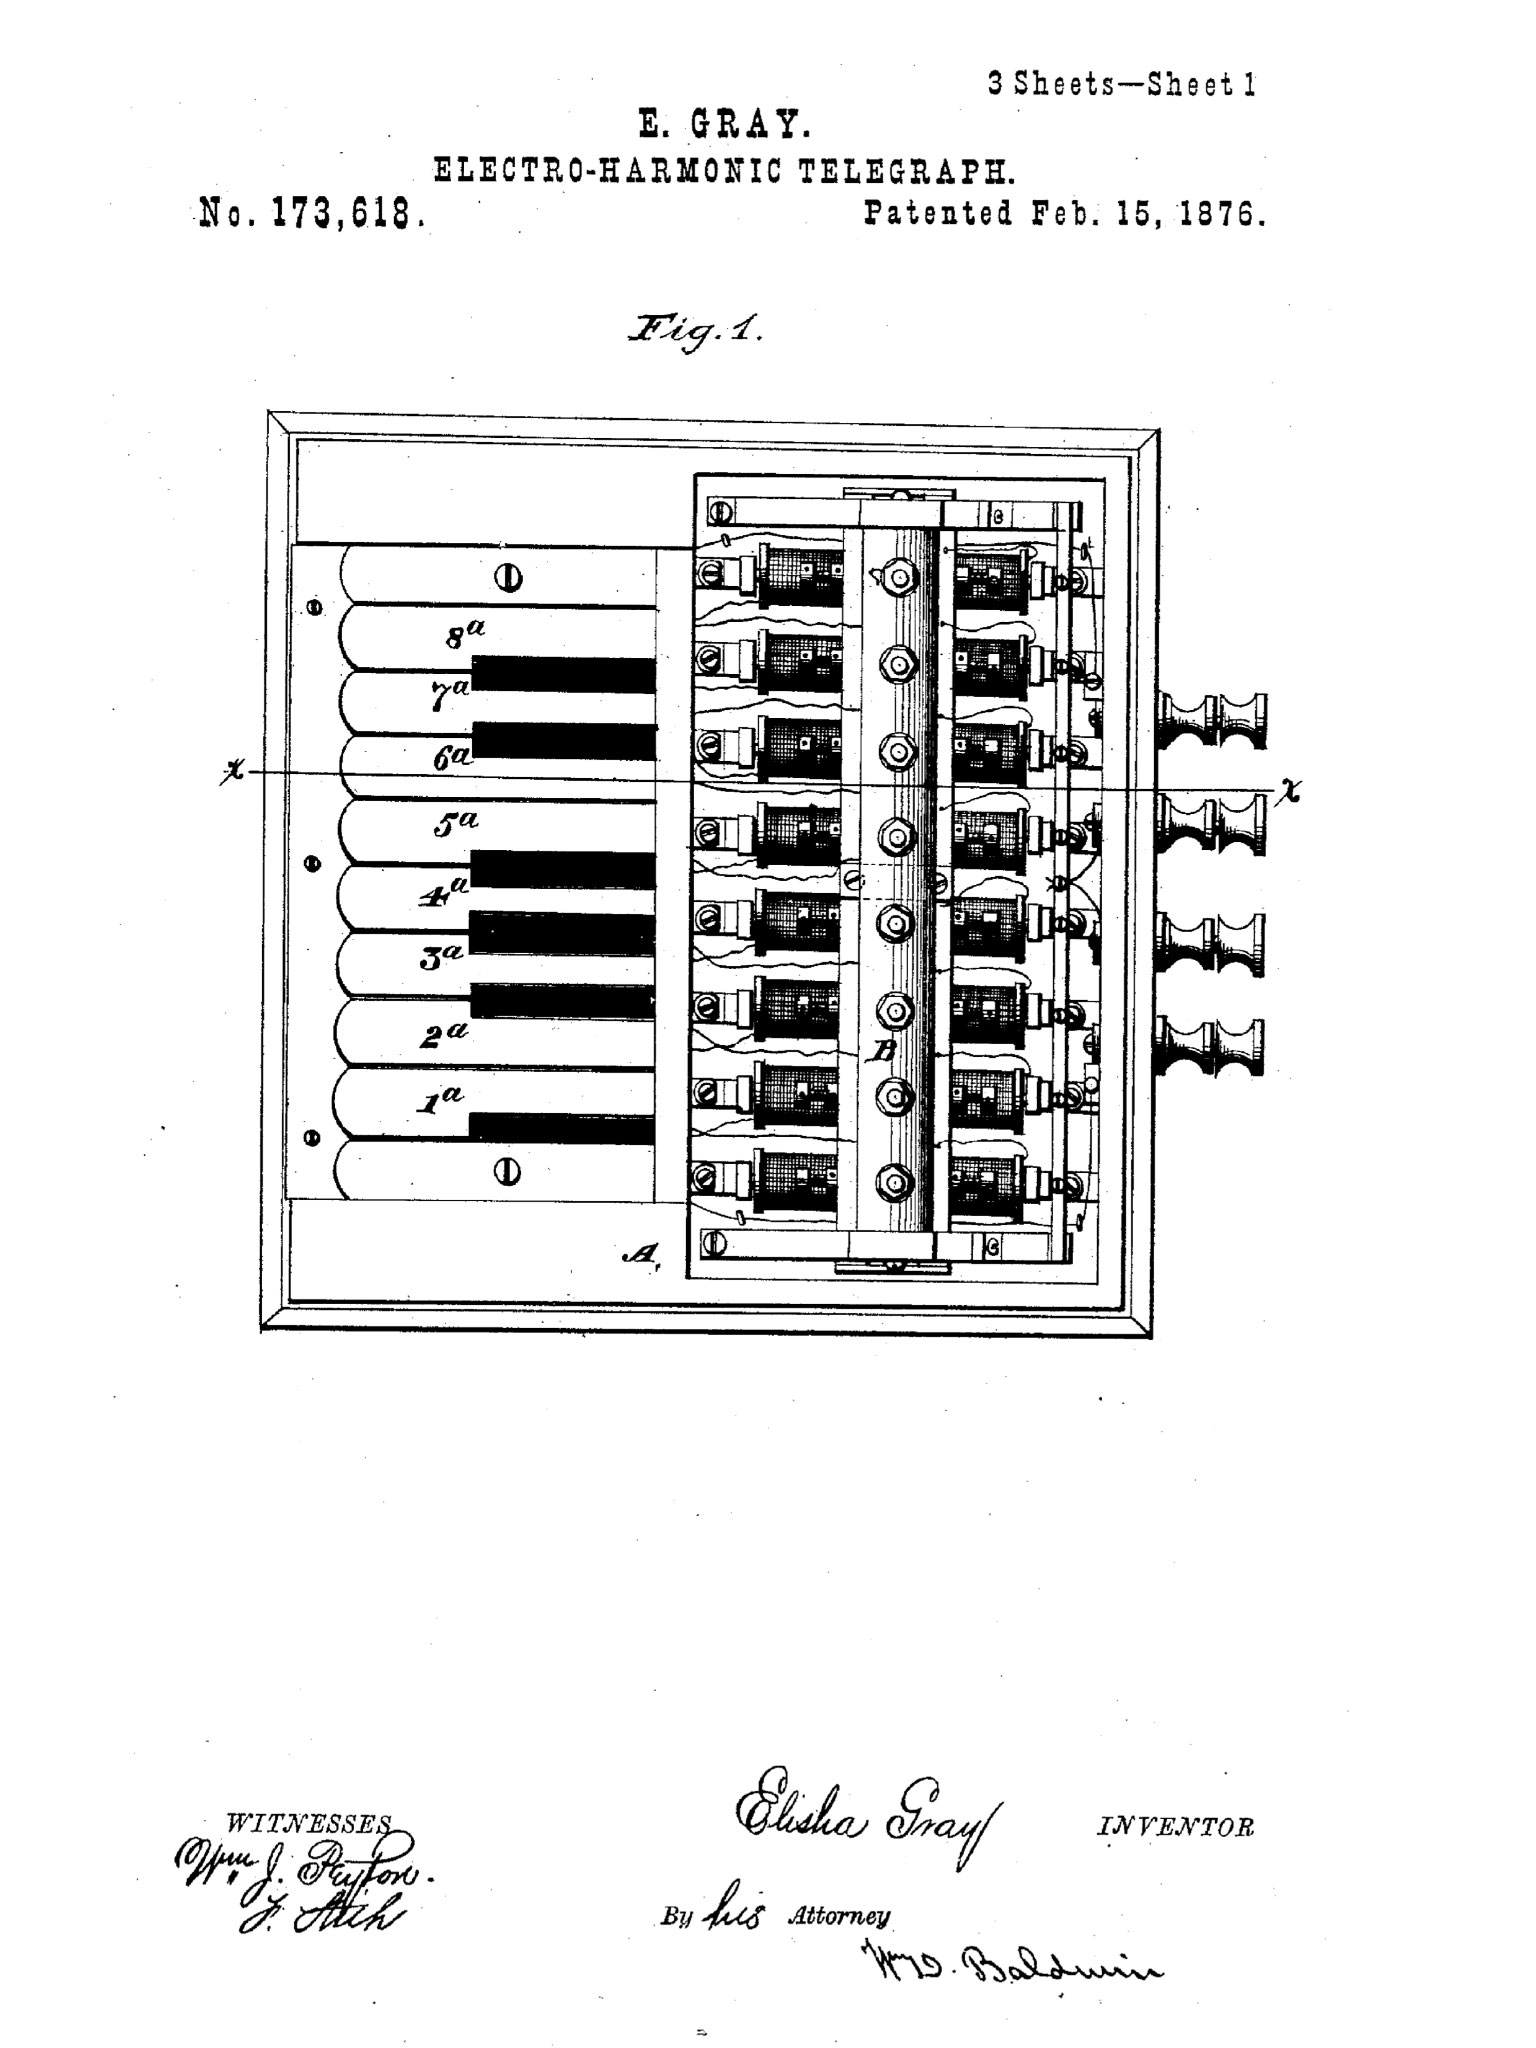
\includegraphics[width=.5\textwidth]{mustel}
	\end{figure}
	
\paragraph{William Dudell}

	William Duddell’s 1899 ``singing arc'' offered pitch control for the audible hum of carbon-arc light bulbs. Here again, the musical application was coincidental - he was originally trying to get rid of the unwanted buzzing sound \citep{nasmyth1908,holmes2002}. 
	
	\begin{figure}[h!]
	  \caption{Illustration of the singing arc}
	  \centering
	    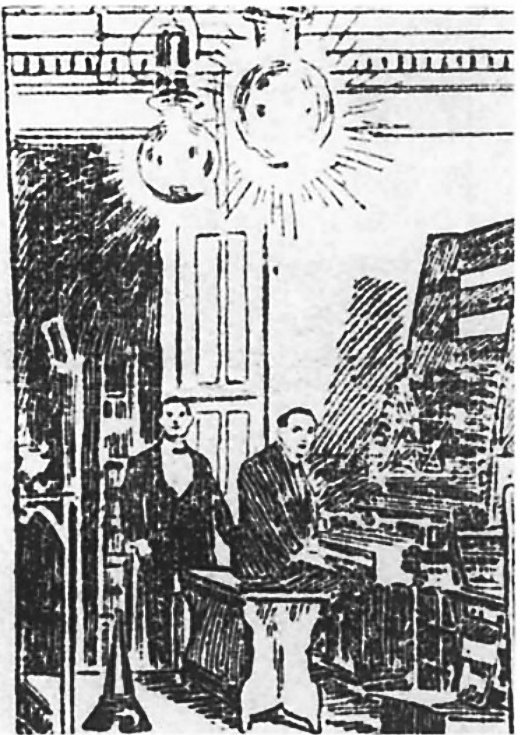
\includegraphics[width=0.5\textwidth]{singarc}
	\end{figure}

\paragraph{Thaddeus Cahill}

	Thaddeus Cahill’s Telharmonium, patented in 1896, was the first successful massive undertaking of electronic music hardware. In its full form, the two-hundred ton instrument was a sophisticated electro-mechanical polyphonic instrument, developed and assembled for the sole purpose of entertainment. With Cahill rises the persona of musical inventor as businessman, effectively becoming one of handmade electronic music’s earliest father figure \citep{holmes2002}. 
	
	\begin{figure}[h!]
	  \caption{Some of the Tellharmonium's tonewheels}
	  \centering
	    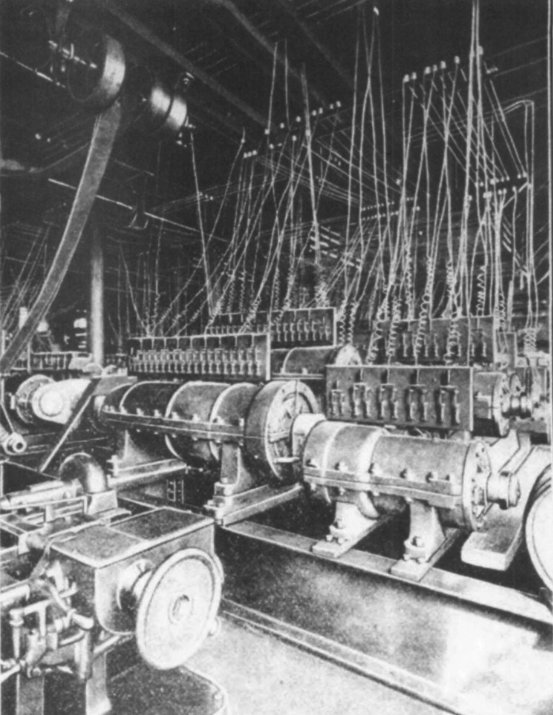
\includegraphics[width=0.5\textwidth]{dynamo}
	\end{figure}

	This short list describes only some of the inventors who were much comfortable with raw materials and physical experimentation than most of today’s electro-acoustic or digital music community. Interestingly enough, none of the signal generation methods described above (electromagnetic oscillation, RLC-circuit oscillation, spark-gap oscillation, electromechanical oscillation) are common in the following generations of electronic music hardware experiments. 

	With electronics still in their infancy - no design tradition, few formal structures -  experimentation is the only option. By operating in an effectively anelectronic context, Cahill and his peers established the baseline for electronic creativity. This is the origin of electronic music, where the promise of the new medium was enough for people to blindly experiment. 

\section{Electronic music as an institution}

In the period following the first world war, the popularization of radio went with the development of not only standardized parts, but also of hobby electronics. It was more cost-effective to buy a kit and build a radio yourself rather than purchase the completed product. In 1922, a Freshman “masterpiece” radio cost \$17 as a kit, while a completed set cost \$60. This corresponds to \$240 v. \$850 in 2014 (radioblvd.com, w2014; data.bls.gov, w2014). 

	\begin{figure}[h!]
	  \caption{advertisement for the Freshman radio kit}
	  \centering
	    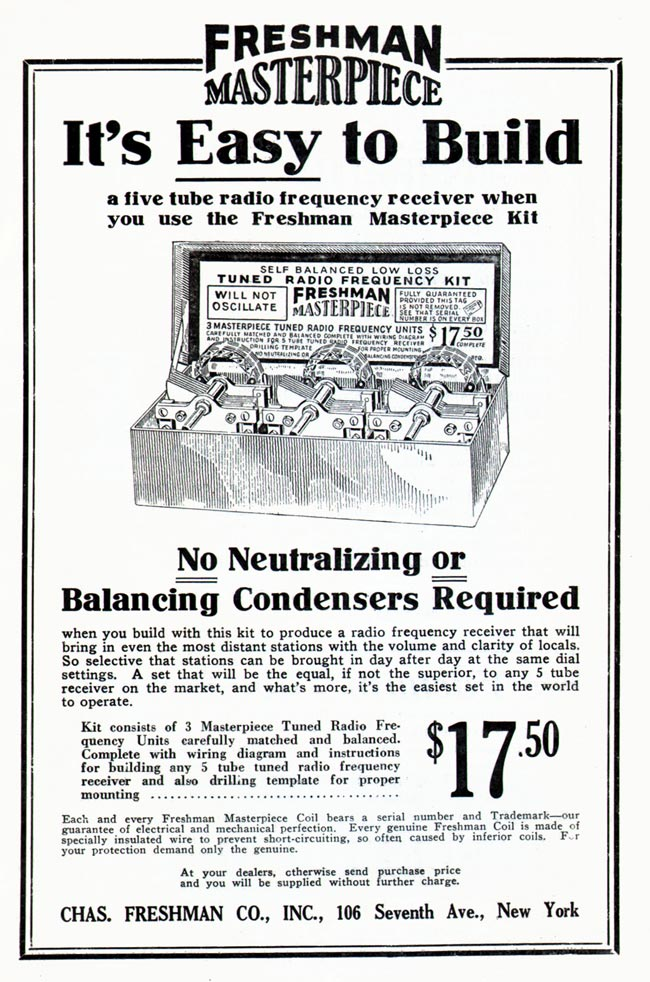
\includegraphics[width=.5\textwidth]{freshman}
	\end{figure}

This was facilitated in the U.S.A. by companies like Radio Shack and Allied Electronics. Both companies, amongst many, sell the parts - resistors, inductors, capacitors, transformers, tubes - and the tools necessary to assemble a variety of consumer audio and radio electronics. 

Radio Shack’s first catalog (w2014) from 1939, contained 80\% kits, parts and tools and 20\% completed products. The increasing availability of parts and tools solidified after the second world war, with catalogs like Radio Shack’s growing from 1939’s 72 pages to 110 in 1946. Heathkit, a major electronics kit focused on high fidelity audio and radio equipment, was founded in 1947. Popular Electronics \#1, which compiled articles on those kits and the various technological developments available to the patient home-builder, was published in 1954. 

	\begin{figure}[h!]
	  \caption{Front cover of Radio Shack's 1939 catalog}
	  \centering
	    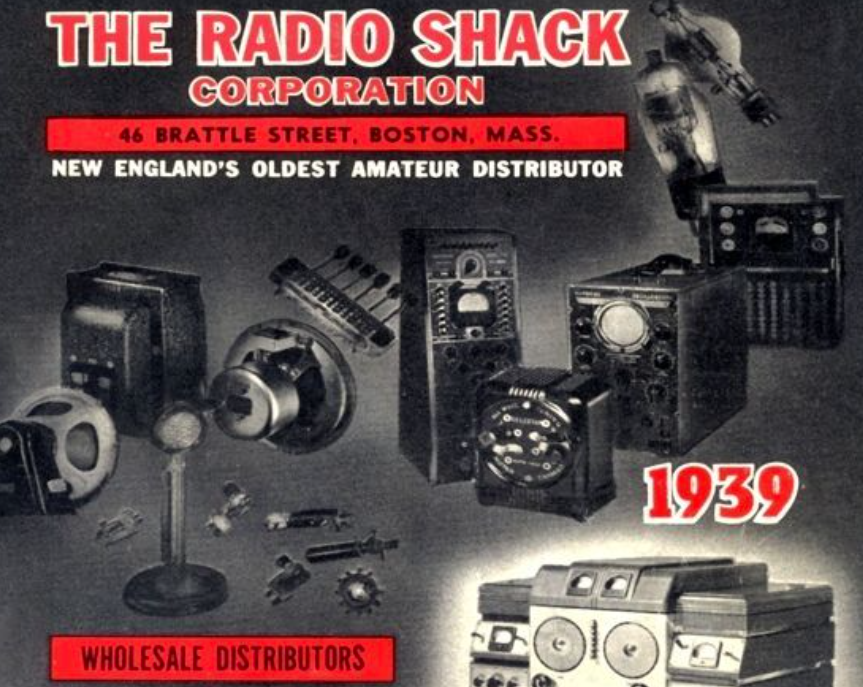
\includegraphics[width=1\textwidth]{radioshack}
	\end{figure}

This resulted in a generation of engineers and musicians growing up with electronics, who were both eager to take advantage of the relatively positive post-war atmosphere \citep{holmes2002}. The father of a certain Robert Moog, whom we will discuss in an upcoming section, was one of the first American amateur radio operators \cite[p.12]{pinch2002}. 

At that time, signal processing was one of the main research areas in the thriving field of electrical engineering. The 1953 edition of the Radiotron Designer's Handbook \citep{langford1953} dedicated a third of its 1500 pages to audio electronics. Schematic, tools, methods and designs are optimized, thoroughly investigated and standardized. Building off their industrial successes, Institutions serve as the breeding ground for most renowned artistic applications of technology. This results in the emergence of the French (ORTF), German (WDR), and Italian (RAI) experimental music studios, all housed by public radio stations. In the U.S., RCA and Columbia University composers collaborated to develop the RCA synthesizer, closer to the telharmonium in scale than anything in the first half of the 20th century. Max Matthews, after being trained as a Navy radio repairman, found work at Bell Labs with music enthusiast John Pierce, whose fostering would mark the beginning of computer music \citep{park2009}. Most of the technology used in those musical systems was a byproduct of the war research effort: it seems natural for the first wave of artists and designers to be involved with those organizations \citep[p.81]{holmes2002}. 

	\begin{figure}[h!]
	  \caption{the RCA Mk.II with its inventors}
	  \centering
	    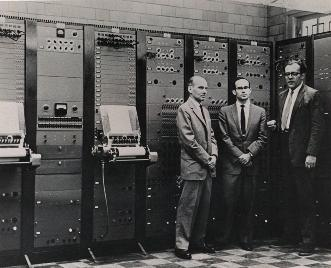
\includegraphics[width=.5\textwidth]{rcamkii}
	\end{figure}

\paragraph{Hugh Le Caine}

Hugh Le Caine’s Electronic Sackbut and its concept of voltage-control proved to be an inspiration for the Moog, and a foreshadow of most electronic music systems. Started in 1945, he worked on the monophonic system until 1971, by which time it possessed two important characteristics: 
\begin{itemize}
	\item the oscillator could be modulated in both timbre and pitch. Furthermore, some settings would create unpredictable variations. Those changes were done through the earliest implementation of voltage control. 
	\item the interface of the instrument allowed for expressivity and ease of use still difficult to achieve today: the piano keys could move side to side to control vibrato, and sense how hard they were pushed down to control amplitude. The left hand that controlled the oscillator parameters did so in way that was particularly rapid to become accustomed to \citep{holmes2002}. 
	
	The Sackbut was a voltage controlled monophonic instrument with specific timbral controls and effective gestural mapping that incorporated controlled amounts of uncertainty. Although it was a failed commercial endeavor, voltage control and touch-sensitivity would emerge in the fifties and sixties as essential components of synthesizers, while impredictability or uncertainty in an instrument would be the concern of Tudor and his cohort. Le Caine sets the example for originality and independence within the institutionalized practice of electronic music and electronic instrument design\cite[p.147]{holmes2002}. 

	\begin{figure}[h!]
	  \caption{Le Caine's Electronic Sackbut}
	  \centering
	    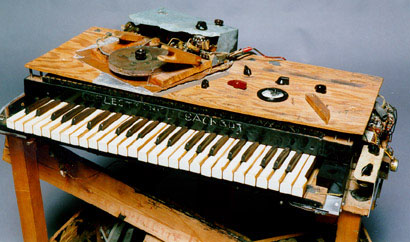
\includegraphics[width=1\textwidth]{sackbut}
	\end{figure}

Le Caine's Sackbut is in the direct continuation of Dudell's experiment - crude electronics combined with the familar keyboard interface. Thoroughly independent research in audio synthesis at the time is limited, but two interesting instances can be presented: 

\paragraph{Raymond Scott}

Raymond Scott was a self-taught hobbyist with the additional motivation, funds and time provided by his successful career as a composer of electronic music for commercials. Having independently developed one of the earliest multi-track tape recorders (7 to 14 tracks), amongst a number of other inventive projects, he would also ultimately receive visits from an impressed Robert Moog. However, he would fail to turn his technological expertise into a successful business. 

As a designer of personal electronic music systems, Scott's vision was most condensed in his \emph{Electronium}. The device is described as being a self-composing device that could be influenced by the user \citep[p.142]{holmes2002}. He sais of the apparatus that is not a synthesizer, as it has not keyboard. By inputting a theme through the hundreds of knobs, permutations on that theme are generated and played - when a satisfactory iteration is produced, the user could activate the record mode and the system would compose independently. ``...the Electronium adds to the composer's thoughts, and a duet relationship is set up between man and machine'' \citep{chusid1999}. The Electronium ``is not played, it is guided''\citep{darter1984}. The device in effect included an analog sequencer and algorithmic composition system, both of which could function together by 1960. 

	\begin{figure}[h!]
	  \caption{Mark Mothersbaugh bought the only electronium from Motown and is restoring it}
	  \centering
	    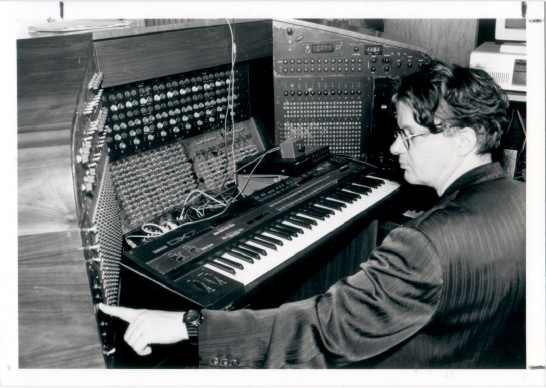
\includegraphics[width=1\textwidth]{electronium}
	\end{figure}
	
Scott's Electronium is an interesting example of independent workers who built off an interest and expertise in science and engineering to push the boundaries of what could musically be done with the available technology. His notorious paranoia with regards to sharing the design (even his attempt at patenting the device failed because of a technicality) meant that little came out of his innovation. From a design perspective, Scott built on the information available to him as a composer and recording engineer to develop his instruments without the technical or financial support of an institution. This is an example of how shared information can still produce advances in instrument design, regardless of whether or not discrete products are shared as well - the open source ecosystem is a robust mechanism that can survive even if it remains static. 

\paragraph{Louis and Bébé Barron}

Louis and Bébé Barron provided soundtracks for films such as 1956’s Forbidden Planet. They were innovative in their implementations of vacuum-tube based synthesis, creating systems based on equations from a cybernetics book by Norbert Wiener. They would describe the resulting devices as ``alive'', an interesting parallel with Scott’s Electronium. In the tradition of Duddell and Gray, the circuits that Louis built were accidently overdriven and eventually failed. These decaying sound processes would be used as the basis for their composition, which they assembled in a way similar to Schaeffer’s concrète process \citep{dunbar2010}.

	\begin{figure}[h!]
	  \caption{Louis and Bébé Barron in the studio}
	  \centering
	    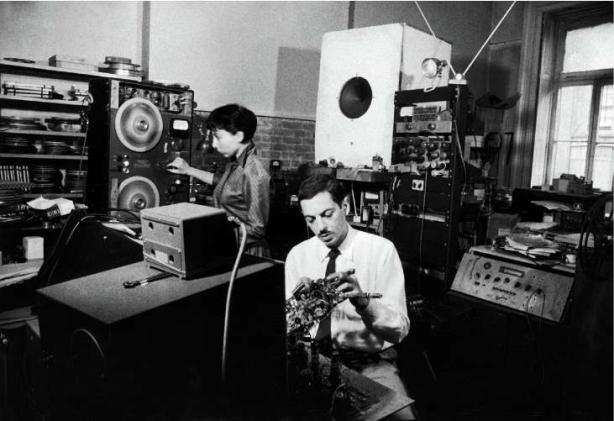
\includegraphics[width=1\textwidth]{barrons}
	\end{figure} 
	
The Barron's and Scott's work, although not immediately influential in terms of instrument design, appear in hindsight as symptoms of the artistic need to tinker and experiment with the concept of electronic music devices as more than tools, but honest instruments if not full-blown artificial composers. Echoes of this intuition will be visible in chapters 3 and 4, as some contemporary practitioners describe there designs as the other half in their musical duets. 

That concept would be explicitly and perhaps more visibly developed by a set of avant-garde musicians in New York City, Michigan and the american west coast. 

John Cage’s experiments throughout the 50’s would incite his collaborator David Tudor to abandon the piano that brought them together in favor of an experimental approach to music through homemade electronics \citep{holzaepfel1994,collins2004}. Unlike our two previous examples, however, Tudor and Cage would have strong affiliations with academia and indirectly, industry. 

As musical systems beneficiated from technological advances developed by the military and major research bodies, fewer people were operating independently with enough success to be documented. Work during the vacuum tube age had undeniable impact: Stockhausen, Schaeffer, Oram, or the Columbia Music Center stand as landmarks in the development of experimental music, arguably solidifying the field as a worthy academic pursuit. However, their efforts were out of the public's possibilities, and often, technical grasp. From a design standpoint, one could describe the ORTF, RAI and WDR studios, as well as the RCA Mk2 as fitting within Dunne's concept of the optimal: an efficient, versatile machine. 

\section{electronic music as a living system}

\subsection{Tudor and Cage: electronics speak for themselves}

	Before being within the reach of the general public, electronic music instruments had to find an audience in that public. In that process, two converging trends contribute to our next development. 
	
	First, the avant-garde continues its exploration of technological possibilities, while reconsidering its limitations and preconceptions. Variations II is a 1960 piece by John Cage, “the greatest degree of abstraction of a compositional and notational model that Cage developed over the period from 1958 to 1961.”
	
\begin{figure}[h!]
  \caption{An instance of setting the score for Cage's \emph{variations II}}
  \centering
    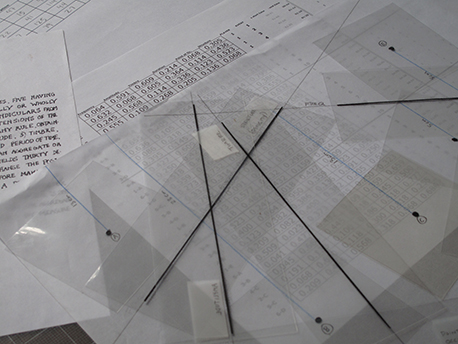
\includegraphics[width=1\textwidth]{variationsii}
\end{figure}
	
	 It was extensively studied, then performed in 1961 by David Tudor, for whom Cage effectively wrote the piece. The extent to which the work was internalized by Tudor has led to some to consider him as the piece’s co-composer \citep{pritchett2004}. It included the use of a complex system of signal processing electronics, designed to implement some of Cage’s ideals of compositional indeterminacy. “You could only hope to influence the instrument”, said Tudor in describing his use of the device \citep{nakai2014}. 
	 
 	\begin{figure}[h!]
 	  \caption{Tudor performing Variations II}
 	  \centering
 	    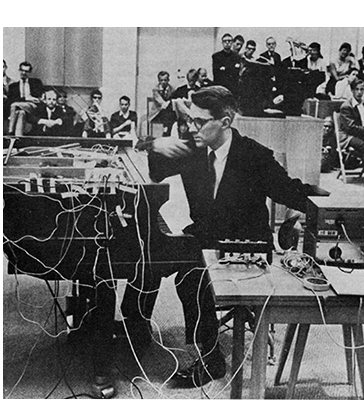
\includegraphics[width=0.5\textwidth]{tudorvar}
 	\end{figure}

Tudor’s debuts are not independent of public or private groups. Fluorescent Sound is commissioned in 1964 by Robert Rauschenberg and sees its sole performance in Stockholm’s Moderna Museet. \emph{Bandoneon!}, his second piece, premiered in 1966’s Nine Evenings of Theatre and Engineering. Instigated by Rauschenberg and facilitated by Bell Laboratories, this event gave artists from the american avant-garde a chance to collaborate with some of the world’s most productive engineers in New York’s Armory building \citep{kuivila2004}. The collaboration would prove instrumental in fostering the experiments in art and technology (EAT) series. 
	
Reminiscent of Barron’s living circuits, Tudor described his second piece as “composing itself out of its own composite instrumental nature.”  \citep{tudor,kuivila2004}. Tudor, through various collaborations, develops an affinity for circuits which ultimately make some of the compositional decisions themselves. 

Cage had been using electronics in performance since the late 30’s, with pieces such as the Imaginary Landscapes series or 1959’s Water Walk. Reich’s 1965 It’s Gonna Rain proved that process-based composition rooted in solely in technology held musical value. Tudor, with his implementation of Variations II, Bandoneon!, and the Rainforest series, legitimizes a compositional approach based explicitly on materiality. “The objects should teach you what it wants to hear”, he states after performing Rainforest IV (1973). Cage will echo the statement in 1987 with the following response: “the components, the circuitry is the music, and it comes alive when it is performed” \citep{nakai2014}. 

Tudor was in a unique position of artistic experience and legitimacy that enabled his experiments to become regarded as groundbreaking and foundational \citep{collins2004}. Through collaborations with Gordon Mumma, David Behrman, Hugh Le Caine, John Fulleman, and John Driscoll, and thorough personal investigation, he gathered enough experience to masterfully implement one of the first documented uses of chaotic electronics in music \citep{kuivila2004}.  Like Cage, he would not be attached to the idea of considering himself a composer \citep{kuivila1998}. Tudor is the model for multiple generations of hobbyists, independent scholars and experimenters who situate themselves somewhere between self-taught artistic systems designer and musician. 

A common thread in Tudor’s work was the spotlighting of electronics customarily hidden during performances, \"composing inside electronics\" ~\ref{appendixA}. In trying to take advantage of the sculptural aspects of the instruments through sonification by using contact microphones or transducers, his work also developed a notion of sound art which challenges the distinction between installation and performance \citep{driscoll2004}. His approach was different from Lucier’s: where the latter focuses each piece on a specific physical phenomenon, Tudor’s work was rarely concerned with minimalist systems \citep{collins2004,driscoll2004}. 

	\begin{figure}[h!]
	  \caption{Performing amidst electronics for \emph{Bandoneon!}}
	  \centering
	    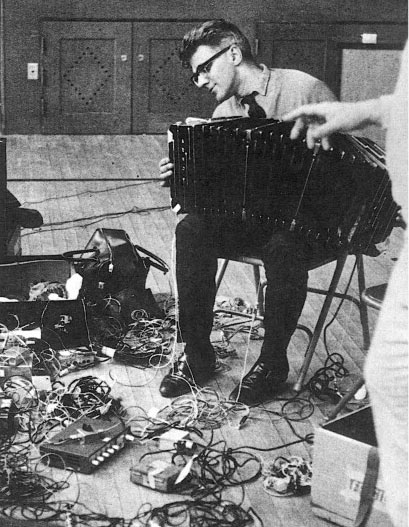
\includegraphics[width=0.5\textwidth]{tudorband}
	\end{figure}

Another manifestation of his originality was his coercion of general-purpose abstraction borrowed from electrical engineering, then adapted for the performance of his pieces and equipment \citep{kuivila2004}. This repurposed set of abstract notations would blur the line between schematic and score, just like Cardew and Earle Brown proposed the use of abstract art as basis for musical performance. In doing so, his performances became more and more personal - Tudor’s oeuvre is “practiced, not preserved” \citep{kuivila1998}. This “musical practice based on constant modification and innovation” \citep{driscoll2004} is a direct foreshadowing of the methods which define online do-it-yourself communities active today. 

	\begin{figure}[h!]
	  \caption{Tudor's diagram for his \emph{Rainforest IV} in effect describes the piece}
	  \centering
	    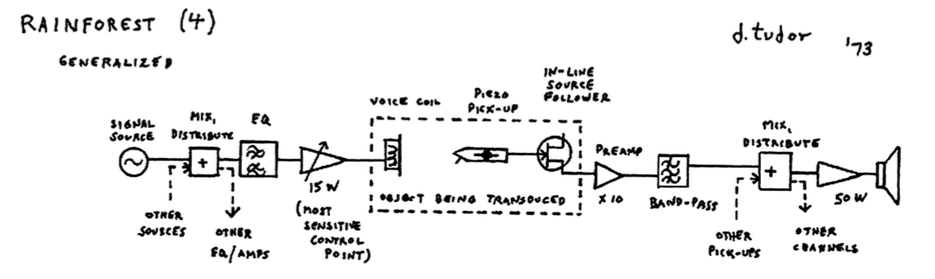
\includegraphics[width=1\textwidth]{rainforest4}
	\end{figure}

	\begin{figure}[h!]
	  \caption{Tudor's score for \emph{Untitled}}
	  \centering
	    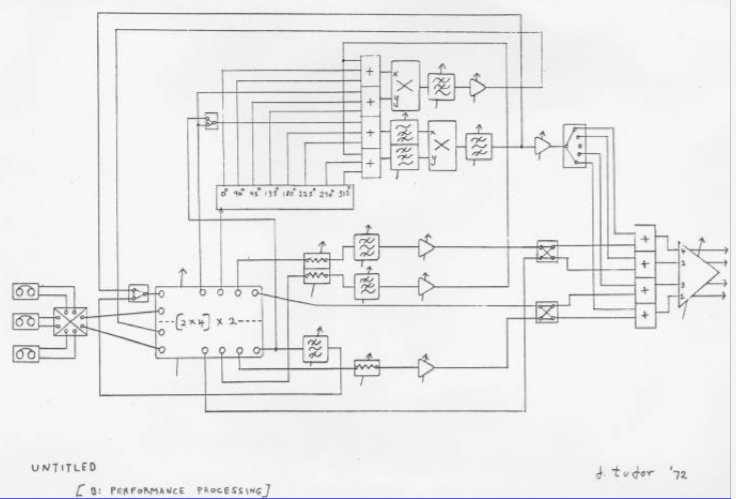
\includegraphics[width=1\textwidth]{untitled}
	\end{figure}

If Tudor defined a practice of experimental electronic music systems that complements Cage’s sonic uncertainty, it is largely thanks to semiconductors (Collins, in\ref{AppendixA}. Transistors and integrated circuits offered the functionality of vacuum tubes without the latter’s size, weight, price and high voltage hazards. These became commercially available and well documented as he started using custom electronics \citep{collins2004}, with Texas Instruments selling their first silicon transistor in 1947 (texas instruments, w2014) and integrated circuits (ICs) becoming available in the 1960’s.  

The easily replaceable, cheaper components would make prototyping musical electronics more accessible, also allowing Tudor to easily enroll help for performances. Starting with 1973’s performance of Rainforest IV, his group of collaborators would solidify as the Composers Inside Electronics group (C.I.E., w2014). The group, reformed for Tudor’s death in 1996 is still active today. Their approach is resumed by Tudor in 1976: 

\begin{quote}
						
Electronic components and circuitry, observed as individual and unique rather than as servomechanisms, more and more reveal their personalities, directly related to the particular musician involved with them. The deeper this process of observation, the more the components seem to require and suggest their own musical ideas, arriving at that point of discovery, always incredible, where music is revealed from ``inside,'' rather than from ``outside.'' \citep{tudor1976,nakai2014}

\end{quote}

Tudor’s innovative methods and C.I.E.’s ever growing cast have guaranteed the relevance of their work in scholarship of musical hardware leading up to the current decade \citep{collins2004,collins2006,collins2008,collins2010,nakai2014,driscoll2004,kuivila2004}. Through the learning, supplying and sharing tools offered online, Tudor’s ideals of experimentation and collaboration have come to be more relevant and accessible than ever. As the E.A.T. experiments failed, the public's appreciation and understanding of overwhelmingly complex electronic art fell \citep{burnham1979}, giving some of the stage to artists who managed to blend adventurous electronics with popular traditions. Voltage control and modular systems became commercially available, giving some leeway to the talented but reclusive experimenters that had not become engineers for Bell Labs or European studios. 

\subsection{The rise of voltage control}

With the development of solid state electronics, audio signal synthesis and processing becomes a more manageable endeavor. As Hugh Le Caine intuited and implemented, but failed to popularize, signals could serve both as raw audio signal or as control information for paramaters of that audio signal. 

Bob Moog, building off of the experience he accumulated assembling, selling and distributing theremin kits, develops that capability in an expensive but publicly available package: the Moog modular synthesizer. Each module serves a primary function and communicates with other modules using those formatted control voltages. The parallel with computer music is straightforward: unit generators are the equivalents of voltage control oscillators (VC0) and their low frequency equivalents (LFO), ring modulation is multiplication, add/substract units are mixers, etc. 

	\begin{figure}[h!]
	  \caption{A schematic for the minimoog's VCO circuit, along with a rough circuit board layout}
	  \centering
	    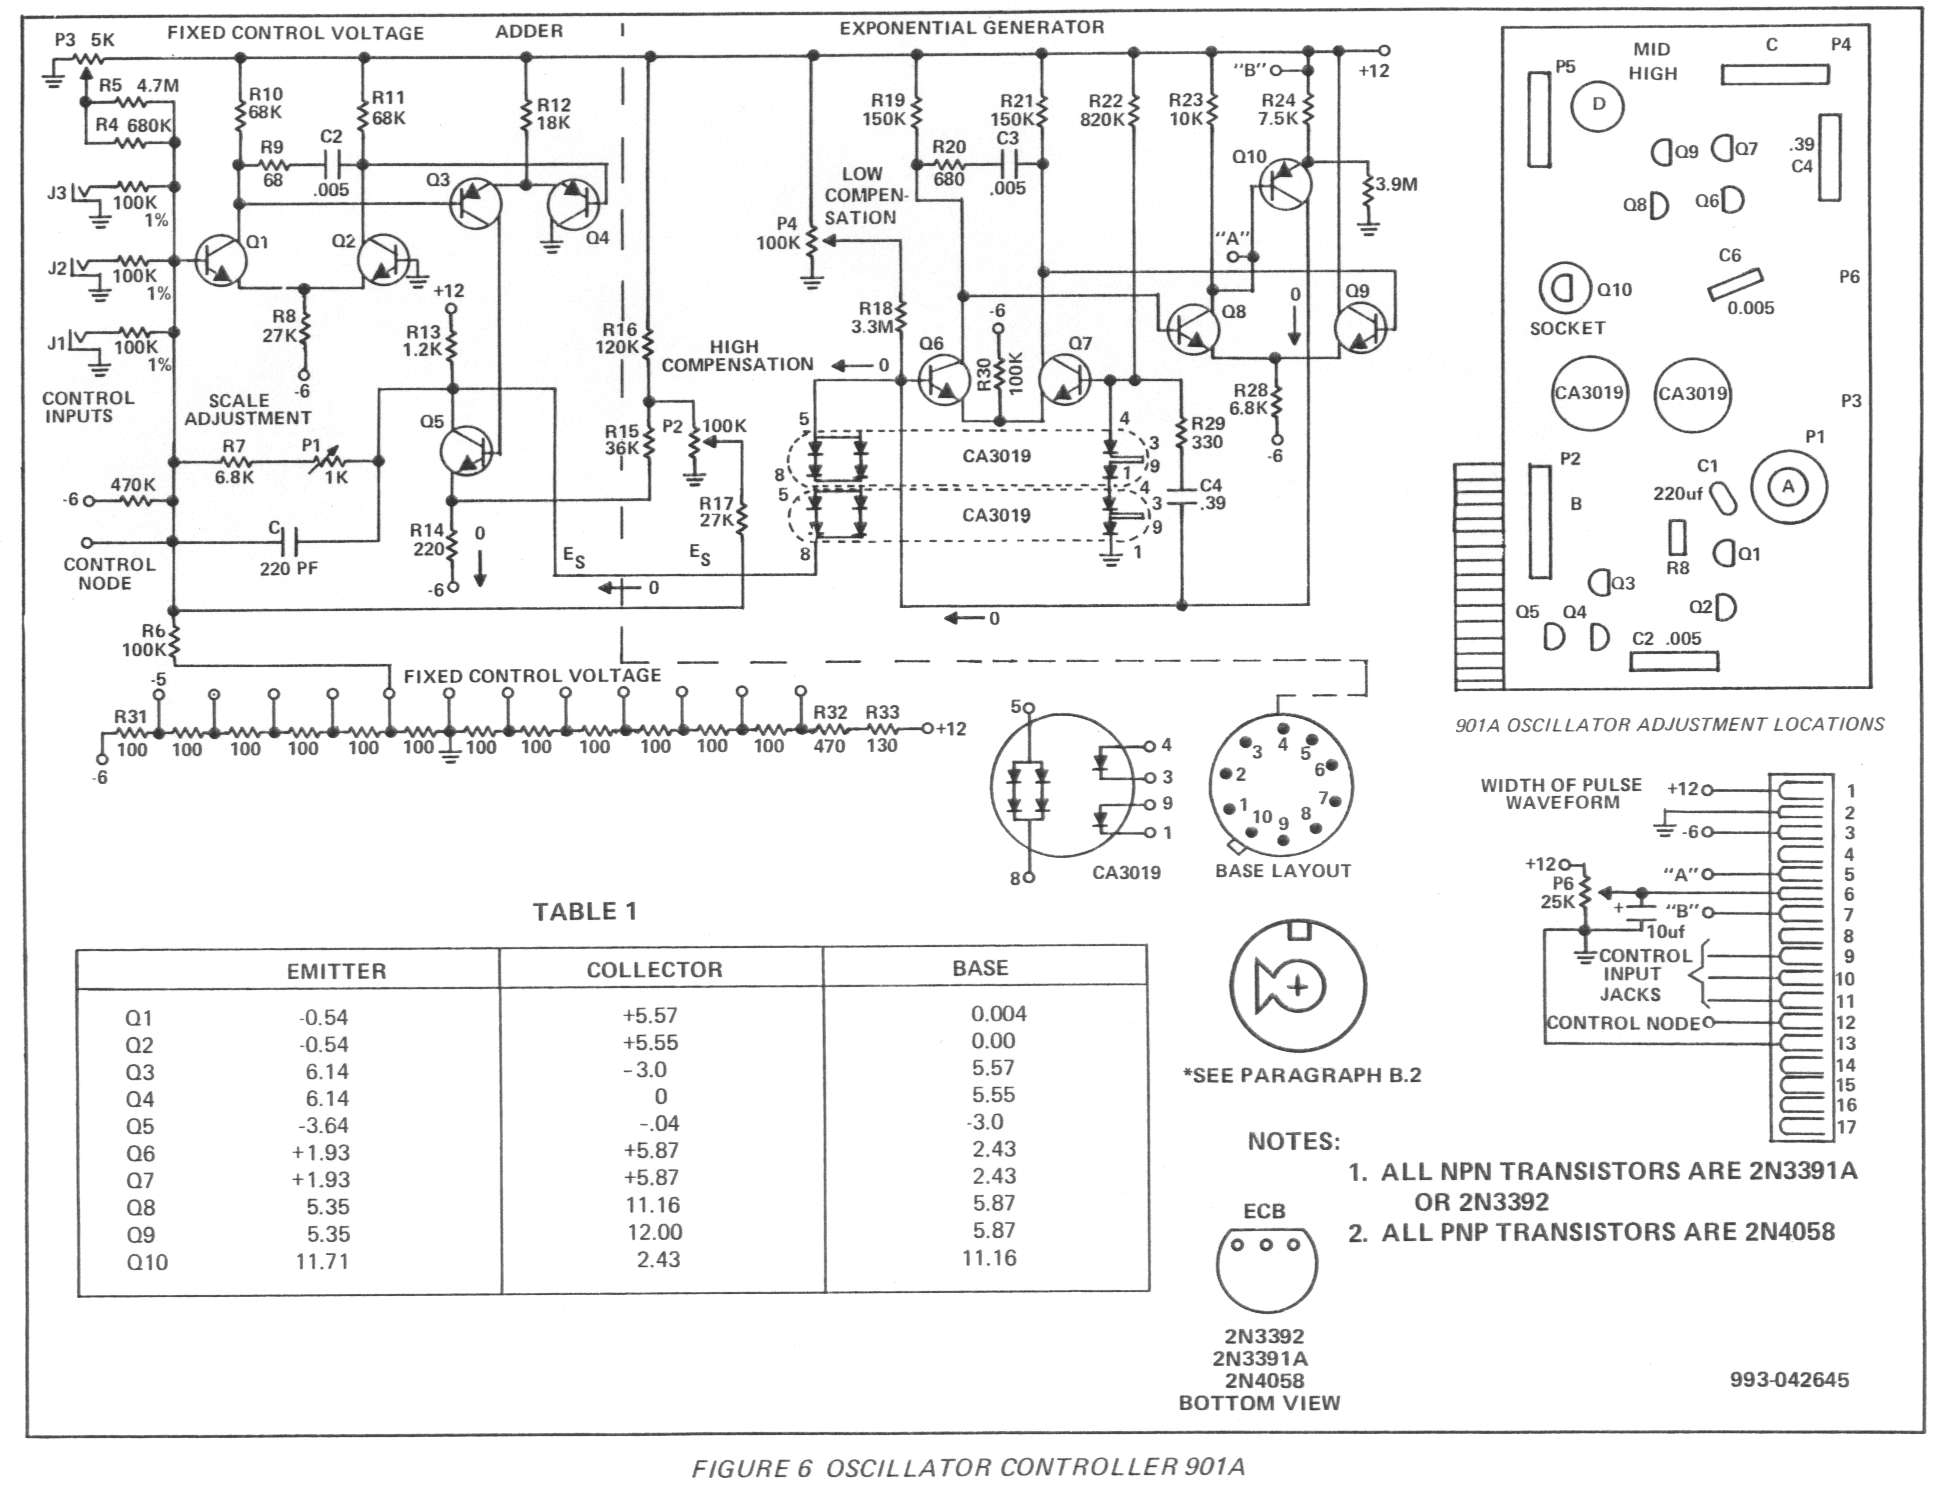
\includegraphics[width=1\textwidth]{minimoogVCO}
	\end{figure}

One can see in the commercial modular synthesizer a first opportunity for the public to ``build'' personalized instruments for popular music. Although the number of modules is limited (not to mention the prohibitive cost), the end user is responsible for the final layout of their device. 

	\begin{figure}[h!]
	  \caption{Klaus Schulze's moog-based system, mid 1970's}
	  \centering
	    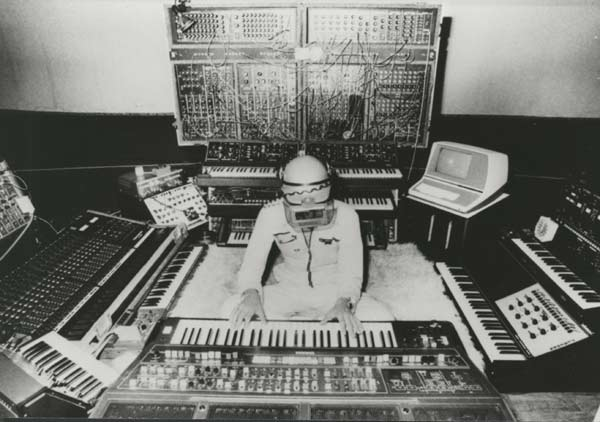
\includegraphics[width=1\textwidth]{schulze}
	\end{figure}

Although Moog is not the only manufacturer of modular systems, the quality of his system, his choice to pair his devices with the more musically familiar keyboard and some public relations skills make him the bridge between classical tape and electronic composers. What Wendy Carlos sees as the tools of ``ugly music'' can now be used for ``appealing music you could listen to.'' \cite[p.169]{holmes2002} As Carlos fine-tuned her own Moog system, she eventually went to get a custom version of the system made to her specifications. 

	\begin{figure}[h!]
	  \caption{Carlos and her Moog 55 system}
	  \centering
	    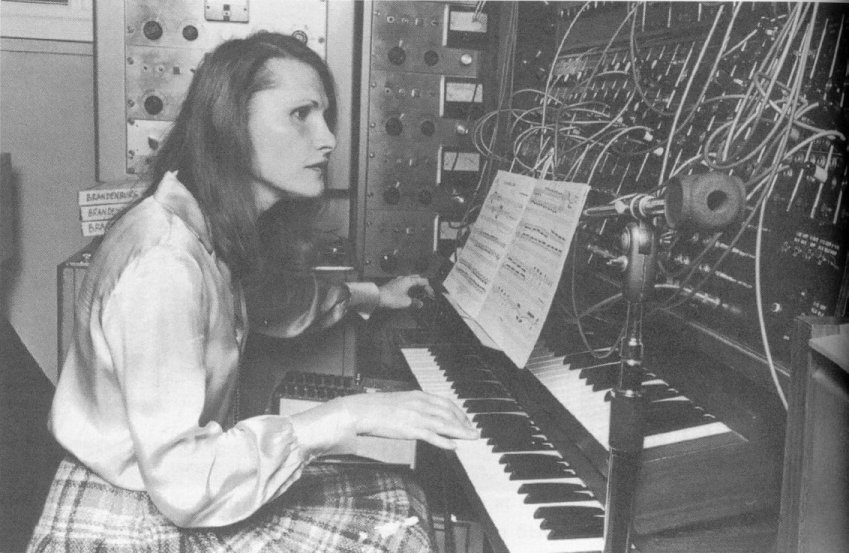
\includegraphics[width=1\textwidth]{carlos}
	\end{figure}

A number of other musically inclined inventors also developed comparable systems, each with their own specificities. Two American complements to Moog are Serge Tcherepnin, designer of the Serge modular system, and Donald Buchla, responsible for the Buchla synthesizer. The latter is most relevant in our discussion. 

As mentioned in the introduction, Buchla viewed himself as a luthier, designer of instruments, rather than the engineer of machines \citep{pinch2001}. His decision to develop new methods of interacting with his circuitry rather than relying on pre-existing schemes like Moog's keyboard severely limited his user-base, but the quality of his luthery would ultimately appear as inspiring for circuit designers up to today \citep{rylan2015}, \ref{AppendixA}. ``The Buchla box was designed for musicians who wanted to produce a complex piece of music in real time.'' \cite[p47]{pinch2002}. If Moog's modular model is the template for much of the additive synthesis audio software and hybrid hardware today, Buchla's interface and interactive system design work are still being digested and re-used. 

	\begin{figure}[h!]
	  \caption{Buchla's distinctive arbitrary function generator (recent model)}
	  \centering
	    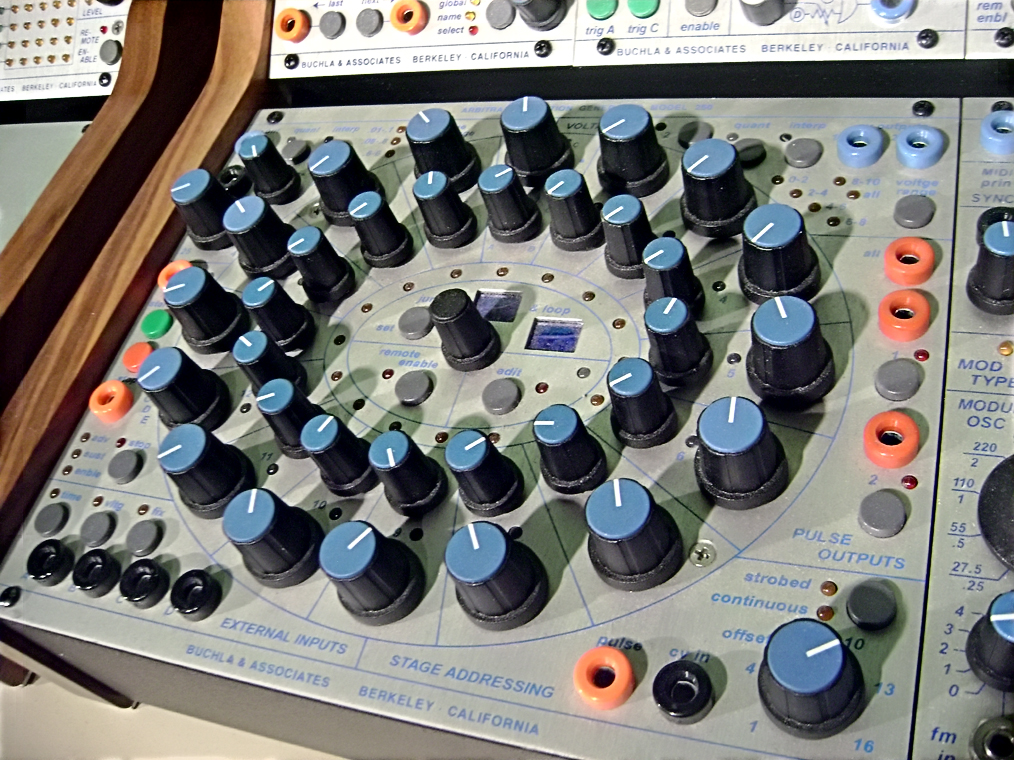
\includegraphics[width=1\textwidth]{buchlaarb}
	\end{figure}

Ultimately, Pinch concludes: ``Designers `script' or `configure' ideal users into their machines.(...) Scripts try to contain the agency of users, but users can exert agency, too, and can come up with their own alternative scripts." \cite[p.311]{pinch2002}. The complex interplay between designer and user takes on a significantly different meaning when those two personas belong to the same person. In that sense, being both the designer of the system and the user allows for more varied processes to emerge, as well as a more original set of parameters for those processes. The ease with which tools permit this dual role directly influences the variety of the instrument design ecosystem and its evolution cycles. 

\subsection{Brian Eno: uncontrolled versus unintentional realizations of music}

A prime example of avant-garde, personal electronic music techniques coming to a popular forefront with relatively little technical support is the British composer Brian Eno and his development of the system later known as \emph{Frippertronics}. His process on \emph{Discreet Music} is clearly related to Tudor's: 

\begin{quote}
	If there is any score for the piece, it must be the operational diagram of the particular apparatus I used for its production. \citep{eno1975}
\end{quote}



\begin{quote}

even though it is correct to say that composing process music does not require electronics, the use of electronic instrumentation often inspires its creation. The very nature of electronic music instruments, old and new, encourages a composer to think in terms of a process, whether that process is a hardwired patch of cables, a virtual patch inside a computer, or the turning of dials to various increments that shape the development of a piece of music. \cite[p.237]{holmes2002}

\end{quote}


If Tudor operated between the component and system levels, Eno is somewhere between system and interaction. However, Tudor's wish to see personality emerge from circuits is echoed by Eno's  ``acceptation of that passive role'' which characterizes the first half of \emph{Discreet Music}. 

This record allows us to briefly discuss the role of intentionality in composition with autonomous or semi-autonomous musical systems. If Eno's practice at that time is implicitly linked to Tudor's, he is also explicitly acknowledging the unintentional nature of his process: 

\begin{quote} ... having laid down, I realized that the amplifier was set at an extremely low level, and that one channel of the stereo had failed completely. Since I hadn't the energy to get up and improve matters, the record played almost inaudibly. This presented what was for me a new way of hearing music - as part of the ambience of the environment.
	
	\citep{eno1975}
	\end{quote}

He combined this new vision of Satie's \emph{Furniture Music} \citep{satie} with an interest for tape-loop based delays dating back to the previous decade, creating the following system: 

\begin{figure}[h!]
  \caption{Operational Diagram for Discreet music}
  \centering
    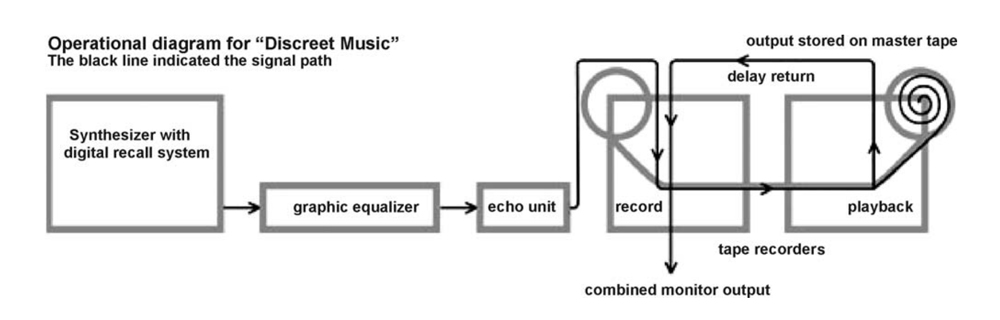
\includegraphics[width=1\textwidth]{discreetdiagram}
\end{figure}

Eno would keep combining this approach to listening with evolved versions of this 1975 system, eventually yielding elements of the \emph{Ambient} series \citep{eno1978,eno1980,eno1980b,eno1982}. This also developed beyond the studio: if \emph{Discreet Music} was originally intended as a backing track for improvisations by Robert Fripp, the latter would eventually use the system extensively through to this day. \emph{Frippertronics} is both a performance, composition and installation medium, a flexible, adaptive and personalized instrument.  

The compelling nature of this release is undeniable. \emph{Discreet Music } holds high value as a prototypical ambient record, an instance of hardware-based process music, and an example of a semi-autonomous electronic music instrument. If Tudor blurred the line between composition and performance through his interpretation of Cage and subsequent live electronics works, Eno's work develops this further by legitimizing curated unintentionality as a compositional prompt. 

More so than Tudor's various devices, \emph{Frippertronics} serve as the archetype of personal electronic music instruments. It illustrates the amount of resources, technical knowledge and musical intuition and luck necessary to make the medium of electronic music one's own. 

At this point, it seems valid to hypothesize that when the ``ideal user'' is the designer, some tend to create systems that have a capacity for independently creating musical material. This hypothesis will be discussed in the upcoming section and chapters.  

\section{Elecronic sound as craft} 

	Tudor as a composer would be largely ignored until his death [Collins, app.A]. As a teacher, he had tremendous impact on what technically inclined artists should or could do. 
	
\subsection{Paul DeMarinis}

Paul DeMarinis worked on the electronics of the 1973 Rainforest IV installation. This period of cohabitation with Tudor's generation of collaborators (John Cage, Robert Ashley, David Behrman) proved to be a formative experience for the Mills College graduate student. Having described them as ``incredibly generous'', they gave him an appreciation of audio electronics that proved to be original for his time. By 1973, he said, ``I wasn't interested in building synthesizers. I was much more interested in building pieces.'' \cite{ouzounian2010}
	
	His first major solo work, the \emph{pygmy gamelan}, has severel important defining features: it was generative, pulling noise from background radiation to produce shifting five-note melodies. It used a combination of early digital and analog ICs, and finally, it wished to ``refer to a culture other than that of high technology.''
	
	 \begin{figure}[h!]
	   \caption{Schematic for \emph{Pygmy Gamelan} \cite[p.107]{beirer2011}}
	   \centering
	     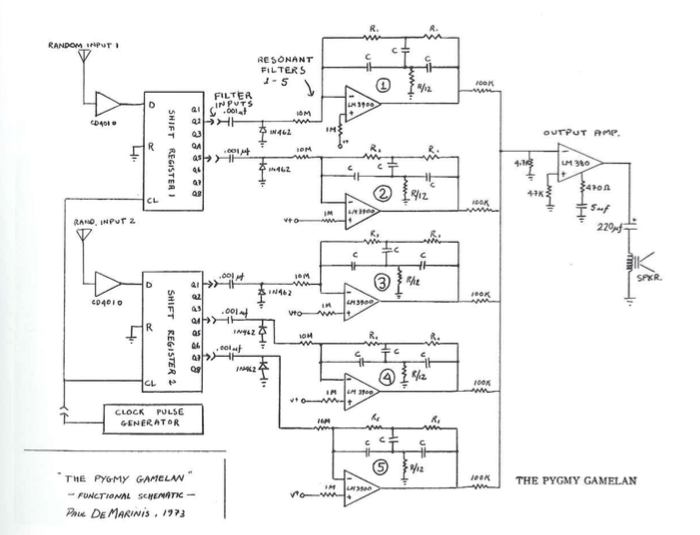
\includegraphics[width=1\textwidth]{pygmyschem}
	 \end{figure}
	 
	 \emph{Pygmy Gamelan}'s importance in our discussion comes from its relative independence from the larger bodies that made it technologically possible \cite[p.27]{beirer2011}. Misuse or re-use of components made for larger consumer devices would prove popular amongst a significant subset of american experimental artists dealing with electronics. 

\subsection{Nic Collins: Handmade Electronic Music} 

Academically, the essence of Tudor’s successors’ would be captured by fellow C.I.E. member Nic Collins. \emph{Handmade Electronic Music} was first published in 2006, presenting an extensive amount of information on homemade electronic instruments with insight from years of experience, references and sources. By completing this project, Collins not only proved that blending academic, commercial and hobbyists attitudes could be successful in all three of those areas, but also linked decades of practices in the do-it-yourself electronic music world to the “maker” movement. The latter started to coalesce around a similar time with publications such as “Make” magazine.

	The values of this book - concepts of imagining, prototyping, assembling from your home - find a strong precedent in pre-industrial craftsmen and the world of boutique electronic music vendors.   \citep{collins2006,ghazala2005,kuivila2004}. 

Although Collins’ introduction hints at the advantages of this approach in the context of electronic music, the advantages of a craft approach to instrument design and fabrication can be further resumed in the potential for personalization, transparency, and skill-transfer \citep{perner2011}. Conversely, the fascination for Collins’ hacking or Ghazala’s more clearly defined circuit-bending can be explained as a desire to fill a need unsatisfied by commercial products \citep{dunne2005}, a process that has shown its ability to serve as the source for entire sub-genres of the musical arts \citep{dunne2005,kelly2009,novak2013}. 
\begin{quote}
“The circuit— whether built from scratch, a customized commercial device, or store-bought and scrutinized to death— became the score.”
\citep{collins2004}
\end{quote}

	Discussing Tudor and Mumma and Kahn, Collins describes the origin of his interest in music hacking, which references the origin of experimental electronics as a legitimate ground for musical composition: 

\begin{quote}
“I learned from Tudor and Mumma that you did not have to have an engineering degree to build transistorized music circuits. David Tudor’s amazing music was based partly on circuits he did not even understand. He liked the sounds they made, and that was enough.” 
- David Berhman \cite[p.ix]{collins2006}  
\end{quote}

\paragraph{the art of hardware hacking}

A look at the structure and content of the work reveals six parts: starting, listening, touching, building, looking, and finishing. Those consist of between two and eight chapters, for a total of 30. Each covers a specific theme such as ``tape heads: playing credit cards'' or ``a little power amplifier: cheap and simple'', revolving around a few schematics, diagrams, guidelines and suggestions for implementations. Historical background is added when appropriate (``David Tudor and Rainforest'', p40; ``Circuit Bending'', p91…). 

There are more pictures than schematics, and what should be striking to anyone already familiar with building electronics is that there rarely are any values or names for parts in schematics - another consequence of Tudor irreverently defacing the key document of electrical engineering. Devising 264 pages of electronics for music involving solely circuits simple enough to describe in a few lines of text appears as a feat in itself. 

	\begin{figure}[h!]
	  \caption{Collins' Light Controlled Mixer circuit}
	  \centering
	    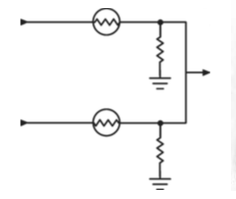
\includegraphics[width=0.3\textwidth]{lightmix}
	\end{figure}

The self-deprecating “keep it stupid” attitude of the introduction rapidly turns into rules number 1 and 2 of hardware hacking, “Fear not!” and “don’t take anything apart that plugs into the wall” (p225). In other words, an electromechanical understanding of electronic music is empowering, and you should experiment as long as you do not risk hurting yourself. This hints at another trope of the open hardware movement, mentioned in the introduction: simple, homemade hardware facilitates sharing and learning, thereby encouraging its practice.

\begin{quote}

“Finally Tim-Berner’s Lee birthed the World Wide Web and a hundred Fuzztones flowered.” 
	
\cite[p211]{collins2006}

\end{quote}

This book can almost serve as an entirely self-contained introduction to electronics in music (falling just short of a soldering iron and a speak \& spell). Collins however made sure that it also is aware of the resources that can compliment it through a list of printed hyperlinks that is fairly exhaustive for its time. In that sense, “Handmade…” also relates to more general current practices in open hardware design. Indeed, it is precisely the open sharing platforms allowed by the world wide web that have fostered the communities which collectively comprise the maker movement. The appendices also reflect loosely broad categories of resources important to both practices: previous documented work. Appendix B appears in retrospect as a paper instructables or hackaday, if every project was hosted on a different homepage. Resources for buying parts and tools are listed in appendix C, where the essentials have not changed and already included allelectronics, jameco, and radioshack. Finally, inspiration: appendix E describes the tracks on CD sold with the book and appendix D lists the rules of hardware hacking and the avant-garde. 
	
	Before discussing the influence of Collins’ book on following publications in related books and articles, it seems important to mention the availability of the book in various digital forms. The original draft for the book, a compilation of class notes, is freely available for download off of the author’s website (w2014). The first result for “handmade electronic music pdf” on most search engines will give a pdf of book.

	By tolerating or passively encouraging open access to resources, Collins contributes directly to the community he has helped shape. More than writing the book on hardware hacking for non-engineers, he’s an essential force in making open hardware design the self-sustaining cycle it aspires to be through the maker movement. By publishing this through a large company while in a professional academic and musical position, he also lends the weight of a more widely recognizable figure to a movement and methodology that challenges the necessity for those very institutions.

\paragraph{impact}  

\begin{quote}

“Collins’s Handmade Electronic Music details many ways in which human interaction can be built into music and sound making devices.” \citep{mills2010}

\end{quote}

	Measuring the influence of this book through simple academic metrics, such as the number of times it is cited in publications following it \citep{harzing2008} yields the following results. “Handmade…” seems to have been referenced in 88 publications (google scholar). For comparison, Road’s “Computer Music Tutorial”, published 10 years earlier, returns 1267 citations, the “Art of Electronics” (a standard circuit design text from 1989) returns 3640, and Gharzala’s “Circuit Bending” from 2005 returns 45. 

	When it is cited, “Handmade…” is rarely commented upon directly. It is referred to in surveys of contemporary sound art, music, and music technology practices \citep{kelly2011,mills2010,pigott2011,rodgers2010}, and as an inspiration in the development of a specific musical controller \citep{ariza2007,hoadley2010,murphy2010,riis2013,valle2011}.
	
	Overall, the academic impact of the work is fairly confined to the field it wished to solidify (music hardware hacking). Its varied content originated from a set of lecture notes, which have since found their place in other college level classes at other institutions. 

On a community level (“do-it-with-others”, diwo, or “do-it-together”, dit), Collins’ impact is difficult to measure objectively. Highly frequented music hardware hacking forums such as Experimentalist Anonymous, diystompboxes, freestompboxes.org, and electro-music.com all contain mention and praises for the accessibility and simplicity of “Handmade…”, but results usually number between 5 and 50. As a reference, searching for Ray Wilson’s popular “music from outer space” do-it-yourself synthesizer website returns between two to three times more results. Collins’ website numbers the quantity of workshops he’s given based on the book since 2004 to “dozens”, meaning that a significant portion of the sharing could still be happening in-person.  

This appears as indicative of the last, and arguably most important point about homemade electronic music instrument design as part of more general arts and crafts \/ diy \/ maker movements. They are fueled by personal engagement and, more importantly, passion. In those circumstances, theorizing, documenting and commercializing is not the priority of the majority but rather the work of the few who turn their passions into a viable working position. 

\section{re-commercializing diy: the maker movement}  

The latest iteration of homemade electronics culture, the maker movement, is described as a third industrial revolution (The Economist, w2014). Here, Fab Labs, modelled after MIT’s NSF-funded center for bits and atoms, allow the public to benefit from some of the efforts of academia to give fabrication a place in everyone’s lives \citep{padfield2014,blikstein2013}. Through this democratization of invention \citep{blikstein2013}, diy culture expands its reach from sunday inventors and engineers to a wider audience. 

In this context, the idea of open source hardware is essential. 

	Often, compelling uses of rapid prototyping (3D printers, cnc mills and other computer assisted manufacturing techniques) are artistic. D-Shape’s large-scale concrete 3D printer is advertised using a sculpture by Andrea Mongante’s Shiro Studio (Shiro Studio w2014). Makerbot’s frontpage for the replicator displays a picture of the device with a completed red plastic bunny on the extrusion platform - this use falls in the artistic range rather than the utilitarian. 

In June 2014, the White House held a maker faire, with president Obama declaring June 18th “National Day of Making” (White House, w2014). Of the 20 projects displayed on the event’s website, 9 were artistic (including 2 instruments: a violin and a banana-synthesizer), and most displayed some level of aesthetic concern. If the third industrial revolution is a democratization of invention, is that the place the arts (and specifically, sound devices) will have? Does a modern version of 9 Evenings exist, and if not, what would it look like? 

On the sidelines of the maker movement, the technology has changed (shifting to digital or mixed-signal systems) along with its means of delivery. Radio Shack and its ilk have lost most of their importance, with online suppliers like Jameco, Digikey and Mouser providing large parts catalogs. Specialized marketplaces like sparkfun and seeedstudio occupy more hobbyist-oriented markets. To compare, by 1970, a Radioshack catalog offered one or two pages , or around .5\% of the catalog for kits, while thirty pages (20\%) are dedicated to parts. In 2002, the last year the company offered catalogs, it contained 25 out of 450 pages of parts, and no kits. The company is currently closing 1100 of its 7000 locations. While this is in no way due solely to the maker movement, Radioshack’s slow death or reconversion does mark the end of an era. 

The rise of accessible embedded systems (arduino, maple boards, raspberry pi, beagleboards…) and availability of relatively free music software (pure data, chuck, csound, supercollider…) leaves music hardware often reduced to the role of place holder for more malleable software. This comes with its own set of design principles (user experience / user interface design), resulting in versatile controllers meant to be used with a computer (monome, linnstrument). With wearable circuits comes the ability to turn most of anything into a controller using the plethora of sensors available to today’s tinkerer. 

Regardless of objective efficiency and versatility, interest in analog sound generation and old-fashioned interfaces is commonplace in electronic music \citep{collins2006}. The range of possibilities for musical expression has become significantly more fragmented. Each approach, whether it is controllerism, hacking or analog traditionalism is being pushed to their extremes. In exchange for this splintering, online resources provide better documentation than before.

The main academic platform for music hardware after 2002 is NIME, which shares all proceedings freely. Amateurs can also find more informal information on a collection of public or semi-private forums (diyaudio, electro-music forum), databases for some type of digital format of designs (hylander), and repositories ran by benevolent individuals that sometimes also try to run small businesses (music from outer space, ken stone).

Most general hardware hacking websites (hackaday, instructables, arduino projects site) contain a significant number of audio hardware projects (hackaday audio, instructables audio, arduino audio forum). It could be said the tools and knowledge necessary for audio hardware designs are more accessible to anyone with an internet connection and the time to teach themselves electronics and programming. In addition, academia is heavily advertising the potential of open source design and manufacturing tools. However, there is very little organized measure or monitoring of the reach of these technologies. Do they truly beneficiate learners and beginners, or do they simply empower some artists and scientists already working on similar projects? Do they only reach people in higher education or with a higher education, or do they attract mostly people already interested in open access technologies? 

The following sections cover two methods of inquiry for these questions. First, recent projects and a series of interviews with their authors allow us to get a snapshot of current practices. Secondly, responses to those projects are devised and documented. An analysis of the process and the efforts undertaken to share those designs follows.

% ---------------
% To incorporate in this chapter
\begin{unsortedStuff}	
\section*{(TO INCORPORATE)}
	\begin{itemize}
		\item 
	\end{itemize}
\end{unsortedStuff}
		
%Blank page to add written thoughts
\begin{optBlankSpace}
	\newpage
	\mbox{}
\end{optBlankSpace}

